\documentclass[]{beamer}

% \usetheme{metropolis}

\usepackage{amsmath}
\usepackage{amssymb}
\usepackage[scale=2]{ccicons}
\usepackage{appendixnumberbeamer}
\usepackage{booktabs}
\usepackage[scale=2]{ccicons}
\usepackage[toc,page]{appendix}
\usepackage{subfigure}
\usepackage{graphicx}
\usepackage{xspace}
\usepackage{adjustbox, lipsum}
\usepackage{bbm}

% Adapted from code originally written by Emtiyaz Khan.

\newcommand{\argmax}{\mathbf{argmax}}
\newcommand{\argmin}{\mathbf{argmin}}

\newcommand{\expect}{\mathbb{E}}

\newcommand{\cS}{\mathcal{S}}
\newcommand{\cA}{\mathcal{A}}

\newcommand{\myvec}[1]{\mbox{$\mathbf{#1}$}}
\newcommand{\myvecsym}[1]{\mbox{$\boldsymbol{#1}$}}

\newcommand{\vzero}{\mbox{$\myvecsym{0}$}}
\newcommand{\vone}{\mbox{$\myvecsym{1}$}}

\newcommand{\valpha}{\mbox{$\myvecsym{\alpha}$}}
\newcommand{\vbeta}{\mbox{$\myvecsym{\beta}$}}
\newcommand{\vchi}{\mbox{$\myvecsym{\chi}$}}
\newcommand{\vdelta}{\mbox{$\myvecsym{\delta}$}}
\newcommand{\vDelta}{\mbox{$\myvecsym{\Delta}$}}
\newcommand{\vepsilon}{\mbox{$\myvecsym{\epsilon}$}}
\newcommand{\veta}{\mbox{$\myvecsym{\eta}$}}
\newcommand{\vgamma}{\mbox{$\myvecsym{\gamma}$}}
\newcommand{\vmu}{\mbox{$\myvecsym{\mu}$}}
\newcommand{\vlambda}{\mbox{$\myvecsym{\lambda}$}}
\newcommand{\vLambda}{\mbox{$\myvecsym{\Lambda}$}}
\newcommand{\vLambdaBar}{\mbox{$\overline{\vLambda}$}}
\newcommand{\vrho}{\mbox{$\myvecsym{\rho}$}}
\newcommand{\vphi}{\mbox{$\myvecsym{\phi}$}}
\newcommand{\vPhi}{\mbox{$\myvecsym{\Phi}$}}
\newcommand{\vpi}{\mbox{$\myvecsym{\pi}$}}
\newcommand{\vpsi}{\myvecsym{\psi}}
\newcommand{\vPsi}{\mbox{$\myvecsym{\Psi}$}}
\newcommand{\vtheta}{\mbox{$\myvecsym{\theta}$}}
\newcommand{\vTheta}{\mbox{$\myvecsym{\Theta}$}}
\newcommand{\vsigma}{\mbox{$\myvecsym{\sigma}$}}
\newcommand{\vSigma}{\mbox{$\myvecsym{\Sigma}$}}
\newcommand{\vOmega}{\mbox{$\myvecsym{\Omega}$}}
\newcommand{\vtau}{\mbox{$\myvecsym{\tau}$}}
\newcommand{\vxi}{\mbox{$\myvecsym{\xi}$}}

\newcommand{\va}{\mbox{$\myvec{a}$}}
\newcommand{\vb}{\mbox{$\myvec{b}$}}
\newcommand{\vc}{\mbox{$\myvec{c}$}}
\newcommand{\vd}{\mbox{$\myvec{d}$}}
\newcommand{\ve}{\mbox{$\myvec{e}$}}
\newcommand{\vo}{\mbox{$\myvec{o}$}}
\newcommand{\vi}{\mbox{$\myvec{i}$}}
\newcommand{\vf}{\mbox{$\myvec{f}$}}
\newcommand{\vg}{\mbox{$\myvec{g}$}}
\newcommand{\vh}{\mbox{$\myvec{h}$}}
\newcommand{\vj}{\mbox{$\myvec{j}$}}
\newcommand{\vk}{\mbox{$\myvec{k}$}}
\newcommand{\vm}{\mbox{$\myvec{m}$}}
\newcommand{\vn}{\mbox{$\myvec{n}$}}
\newcommand{\vp}{\mbox{$\myvec{p}$}}
\newcommand{\vq}{\mbox{$\myvec{q}$}}
\newcommand{\vr}{\mbox{$\myvec{r}$}}
\newcommand{\vs}{\mbox{$\myvec{s}$}}
\newcommand{\vt}{\mbox{$\myvec{t}$}}
\newcommand{\vu}{\mbox{$\myvec{u}$}}
\newcommand{\vv}{\mbox{$\myvec{v}$}}
\newcommand{\vw}{\mbox{$\myvec{w}$}}
\newcommand{\vws}{\mbox{$\vw_s$}}
\newcommand{\vwh}{\mbox{$\hat{\vw}$}}
\newcommand{\vx}{\mbox{$\myvec{x}$}}
\newcommand{\vxt}{\mbox{$\myvec{\tilde{x}}$}}
\newcommand{\vy}{\mbox{$\myvec{y}$}}
\newcommand{\vyt}{\mbox{$\myvec{\tilde{y}}$}}
\newcommand{\vz}{\mbox{$\myvec{z}$}}
\newcommand{\vA}{\mbox{$\myvec{A}$}}
\newcommand{\vB}{\mbox{$\myvec{B}$}}
\newcommand{\vC}{\mbox{$\myvec{C}$}}
\newcommand{\vD}{\mbox{$\myvec{D}$}}
\newcommand{\vE}{\mbox{$\myvec{E}$}}
\newcommand{\vF}{\mbox{$\myvec{F}$}}
\newcommand{\vG}{\mbox{$\myvec{G}$}}
\newcommand{\vH}{\mbox{$\myvec{H}$}}
\newcommand{\vI}{\mbox{$\myvec{I}$}}
\newcommand{\vJ}{\mbox{$\myvec{J}$}}
\newcommand{\vK}{\mbox{$\myvec{K}$}}
\newcommand{\vL}{\mbox{$\myvec{L}$}}
\newcommand{\vM}{\mbox{$\myvec{M}$}}
\newcommand{\vN}{\mbox{$\myvec{N}$}}
\newcommand{\vO}{\mbox{$\myvec{O}$}}
\newcommand{\vP}{\mbox{$\myvec{P}$}}
\newcommand{\vQ}{\mbox{$\myvec{Q}$}}
\newcommand{\vR}{\mbox{$\myvec{R}$}}
\newcommand{\vS}{\mbox{$\myvec{S}$}}
\newcommand{\vT}{\mbox{$\myvec{T}$}}
\newcommand{\vU}{\mbox{$\myvec{U}$}}
\newcommand{\vV}{\mbox{$\myvec{V}$}}
\newcommand{\vW}{\mbox{$\myvec{W}$}}
\newcommand{\vX}{\mbox{$\myvec{X}$}}
\newcommand{\vXs}{\mbox{$\vX_{s}$}}
\newcommand{\vXt}{\mbox{$\myvec{\tilde{X}}$}}
\newcommand{\vY}{\mbox{$\myvec{Y}$}}
\newcommand{\vZ}{\mbox{$\myvec{Z}$}}


\usetheme{metropolis}

\setbeamerfont{bibliography item}{size=\footnotesize}
\setbeamerfont{bibliography entry author}{size=\footnotesize}
\setbeamerfont{bibliography entry title}{size=\footnotesize}
\setbeamerfont{bibliography entry location}{size=\footnotesize}
\setbeamerfont{bibliography entry note}{size=\footnotesize}

%Information to be included in the title page:
\title{Standard and Natural Policy Gradients for Discounted Rewards}

\author{Aaron Mishkin}
\institute{UBC MLRG 2018W1}

\begin{document}

\begin{frame}

    \titlepage

\end{frame}

\begin{frame}{Motivating Example: Humanoid Robot Control}

Consider learning a control model for a robotic arm that plays table tennis.

\begin{figure}
    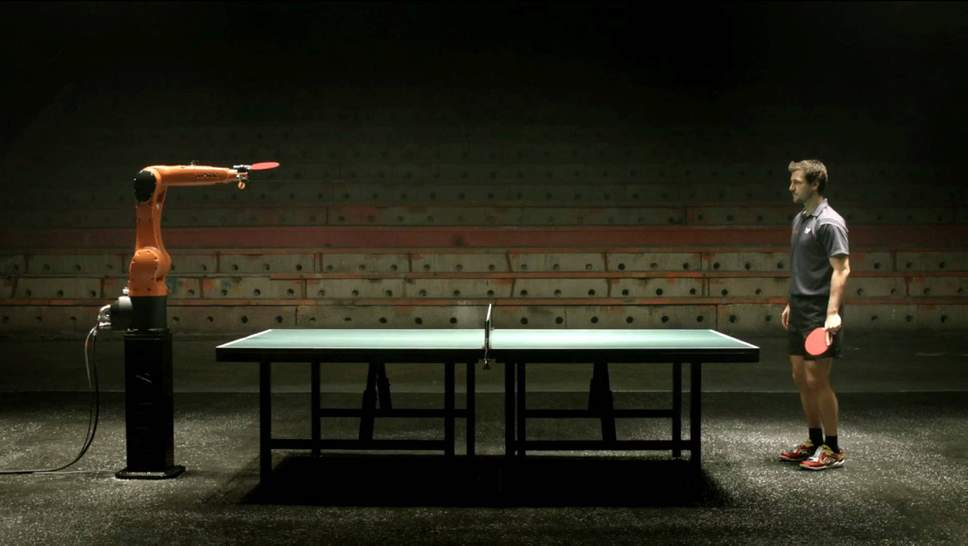
\includegraphics[width=0.8\textwidth]{arm_tennis.jpg}
\end{figure}


{\let\thefootnote\relax\footnote{{\tiny https://static.independent.co.uk/s3fs-public/thumbnails/image/2014/03/11/15/ping-pongv2.jpg?w968}}}

\end{frame}

\begin{frame}{Why Policy Gradients?}
Policy gradients have several advantages:
\begin{itemize}
    \item Policy gradients permit explicit policies with complex parameterizations.
    \item Such policies are easily defined for continuous state and action spaces.
    \item Policy gradient approaches are guaranteed to converge under standard assumptions while greedy methods (SARSA, Q-learning, etc) are not.
\end{itemize}
\end{frame}

\begin{frame}{Roadmap}

    \tableofcontents

    % \begin{enumerate}
    %     \item Background and Notation
    %     % \begin{enumerate}
    %     %     \item Markov Decision Processes
    %     %     \item Polcies and the Bellman Equations
    %     % \end{enumerate}
    %     \item The Policy Gradient Theorem
    %     % \begin{enumerate}
    %     %     \item Original Result
    %     %     \item Extension to Approximate Value Functions
    %     %     \item An Algorithmic Template
    %     % \end{enumerate}
    %     \item Natural Policy Gradients
    %     % \begin{enumerate}
    %     %     \item Background on Natural Gradients
    %     %     \item Derivation and Discussion
    %     %     \item An Algorithmic Template
    %     % \end{enumerate}
    % \end{enumerate}

\end{frame}

\section{Background and Notation}

\begin{frame}{Markov Decision Processes (MDPs)}

A discrete-time MDP is specified by the tuple $\{S, A, d_0, f, r\}$:

\begin{itemize}
    \item States are $\vs \in \cS$; actions are $\va \in \cA$.
    \item $f$ is the transition distribution. It satisfies the Markov property:
    \[ f(\vs_t, \va_t, \vs_{t+1}) = p(\vs_{t+1}|\vs_0, \va_0 ... \vs_t, \va_t) = p(\vs_{t+1}|\vs_t, \va_t) \]
    \item $d_0(\vs_0)$ is the initial distribution over states.
    \item $r(\vs_{t}, \va_{t}, \vs_{t+1})$ is the reward function, which may be deterministic or stochastic.
    \item Trajectories are sequences of state-action pairs: $\vtau_{0:t} = \{(\vs_0, \va_0), ..., (\vs_t, \va_t) \}$
\end{itemize}

We treat states $\vs$ as fully observable.

\end{frame}

\begin{frame}{Continuous State and Action Spaces}

We will consider MDPs with continuous state and action spaces. In the robot control example:
\begin{itemize}
    \item $\vs \in \cS$ is a real vector describing the configuration of the robotic arm's movement system and the state of environment.
    \item $\va \in \cA$ real vector representing a motor command to the arm.
    \item Given action $\va$ in state $\vs$, the probability of being in a \textit{region} of state space $\cS' \subseteq \cS$ is:
    \[ P(\vs' \in \cS' | \vs, \va) = \int_{\cS'} p(\vs'| \vs, \va) d\vs' \]

    Future states $\vs'$ are only known probabilistically because our control and physical models are approximations.
\end{itemize}

\end{frame}

\begin{frame}{Policies}
    Policies defines how an agent acts in the MDP:
    \begin{itemize}
        \item A \textit{policy} $\pi: \cS \times \cA \rightarrow [0, \infty)$ is the conditional density function:
        \begin{align*}
            \pi(\va | \vs) := \text{probability of taking action $\va$ in state $\vs$}
        \end{align*}
        \item The policy is deterministic when $\pi(\va | \vs)$ is a Dirac-delta function.
        \item Actions are chosen by sampling from the policy $\va \sim \pi(\va | \vs)$.
        \item The quality of a policy is given by an objective function $J(\pi)$.
    \end{itemize}

\end{frame}

\begin{frame}{Bellman Equations}

We consider discounted returns with factor $\gamma \in [0,1]$. The Bellman equations describe the quality of a policy recursively:
\begin{align*}
    Q^\pi(\vs, \va) &:= \int_\cS f(\vs' | \vs, \va)\left(r(\vs, \va, \vs') + \int_\cA \pi(\va' | \vs') \gamma Q^\pi(\vs', \va') d\va' \right) d\vs'\\\\
    V^\pi(\vs) &:= \int_\cA \pi(\va | \vs) Q^\pi(\vs, \va) d\va\\
    &= \int_\cA \pi(\va | \vs) \int_\cS f(\vs' | \vs, \va)\left(r(\vs, \va, \vs') + \gamma V^\pi(\vs')\right) d\vs' d\va\\
    &= \int_\cA \pi(\va | \vs) \int_\cS f(\vs' | \vs, \va)r(\vs, \va, \vs') d\vs'd\va \ \\
    & + \int_\cA \pi(\va | \vs) \int_\cS f(\vs' | \vs, \va) \gamma V^\pi(\vs') d\vs' d\va\\
\end{align*}

\end{frame}

\begin{frame}{Actor-Critic Methods}
    Three major flavors of reinforcement learning:
    \begin{enumerate}
        \item Critic-only methods: Learn an approximation of the state-action reward function: $R(\vs, \va) \approx Q^\pi(\vs,\va)$.
        \item Actor-only methods: Learn the policy $\pi$ directly from observed rewards. A parametric policy $\pi_\theta$ can be optimized by descending the \textit{policy gradient}:
        \[ \nabla_\theta J(\pi_\theta) = \frac{\partial J(\pi_\theta)}{\partial \pi_\theta} \frac{\partial \pi_\theta}{\partial \theta} \]
        \item Actor-Critic methods: Learn an approximation of the reward $R(\vs,\va)$ jointly with the policy $\pi(\va | \vs)$.
    \end{enumerate}
\end{frame}

\begin{frame}{Value of a Policy}
    We can use the Bellman equations to write the overall quality of the policy:
    {\small
    \begin{align*}
        &\frac{J(\pi)}{(1-\gamma)} = \int_\cS d_0(\vs_0) V^\pi(\vs_0) d\vs_0\\
        &= \sum_{k=0}^\infty \int_\cS p(\vs_k = \bar \vs) \int_\cA \pi(\va_k | \bar \vs) \int_\cS f(\vs_{k+1} | \bar \vs \va_k) \gamma^k r(\bar \vs, \va_k, \vs_{k+1}) d\vs_{t+1} d\va d \bar \vs \\
        &= \int_\cS \sum_{k=0}^\infty \gamma^k p(\vs_k = \bar \vs) \int_\cA \pi(\va_k | \bar \vs) \int_\cS f(\vs_{k+1} | \bar \vs \va_k) r(\bar \vs, \va_k, \vs_{k+1}) d\vs_{t+1} d\va d\bar\vs
    \end{align*}
    }
    Define the "discounted state" distribution:
    \[ d^\pi_\gamma(\bar \vs) = (1-\gamma)\sum_{k=0}^\infty \gamma^k p(\vs_k = \bar \vs) \]

\end{frame}

\begin{frame}{Value of Policy: Discounted Return}
    The final expression for the overall quality of the policy is the \textit{discounted return}:
    \begin{align*}
        J(\pi) = \int_\cS d^\pi_\gamma(\bar \vs) \int_\cA \pi(\va | \bar \vs) \int_\cS f(\vs' | \bar \vs, \va) r(\bar \vs, \va, \vs') d\vs' d\va d\bar\vs
    \end{align*}
    Assuming that the policy is parameterized by $\theta$, how can we compute the policy gradient $\nabla_\theta J(\pi_\theta)$? \\
\end{frame}

\section{The Policy Gradient Theorem}

\begin{frame}{Policy Gradient Theorem: Statement}
\textbf{Theorem 1 - Policy Gradient:} \cite{sutton2000policy} The gradient of the discounted return is:
\begin{align*}
    \nabla_\theta J(\pi_\theta) &= \int_\cS d^\pi_\gamma(\bar \vs) \int_\cA \nabla_\theta \pi_\theta(\va_k | \bar \vs) Q^\pi(\vs, \va) d\va d\bar\vs
\end{align*}
\textbf{Proof:} The relationship between the discounted return and the state value function gives us our starting place:
\begin{align*}
    \nabla_\theta J(\pi_\theta) &= (1-\gamma) \nabla_\theta \int_\cS d_0(\vs_0) V^\pi(\vs_0) d\vs_0\\
    &= (1-\gamma) \int_\cS d_0(\vs_0) \nabla_\theta V^\pi(\vs_0) d\vs_0\\
\end{align*}

\end{frame}

\begin{frame}{Policy Gradient Theorem: Proof}
    Consider the gradient of the state value function:
    {\small \begin{align*}
        \nabla_\theta V^\pi(\vs) &= \nabla_\theta \int_\cA \pi_\theta(\va | \vs) Q^\pi(\vs, \va) d\va \\
        &= \int_\cA \nabla_\theta \pi_\theta(\va | \vs) Q^\pi(\vs, \va) + \pi_\theta(\va | \vs) \nabla_\theta Q^\pi(\vs, \va) d\va \\
        &= \int_\cA \nabla_\theta \pi_\theta(\va | \vs) Q^\pi(\vs, \va) + \pi_\theta(\va | \vs) \nabla_\theta \int_\cS f(\vs' | \vs, \va) \bigg(r(\vs, \va, \vs') \ + \\
        & \hspace{7cm} \gamma V^\pi(\vs') \bigg) d\vs' d\va \\
        &= \int_\cA \nabla_\theta \pi_\theta(\va | \vs) Q^\pi(\vs, \va) + \pi_\theta(\va | \vs) \int_\cS \gamma f(\vs' | \vs, \va) \nabla_\theta V^\pi(\vs') d\vs' d\va \\
    \end{align*} }
    This is recursive expression for the gradient that we can unroll!

\end{frame}

\begin{frame}{Policy Gradient Theorem: Proof Continued}
    Unrolling the expression from $\vs_0$ gives:
    {\small \begin{align*}
        \nabla_\theta V^\pi(\vs_0) &= \int_\cA \nabla_\theta \pi_\theta(\va_0 | \vs_0) Q^\pi(\vs_0, \va_0) d \va_0 \\
        & + \int_\cA \pi_\theta(\va_0 | \vs_0) \int_\cS \gamma f(\vs_1 | \vs_0, \va_0) \nabla_\theta V^\pi(\vs_1) d\vs_1 d\va_0 \\
        &= \int_\cS \sum_{k=0}^\infty \gamma^k p(\vs_k = \bar \vs | \vs_0) \int_\cA \nabla_\theta \pi_\theta(\va | \bar \vs) Q^\pi(\bar \vs, \va) d\va d\bar \vs
    \end{align*} }
    So the policy gradient is given by:
    \begin{align*}
        \frac{\nabla_\theta J(\pi_\theta)}{(1-\gamma)} &= \int_\cS d_0(s_0) \int_\cS \sum_{k=0}^\infty \gamma^k p(\vs_k = \bar \vs | \vs_0) \int_\cA \nabla_\theta \pi_\theta(\va | \bar \vs) Q^\pi(\bar \vs, \va) d\va d\bar \vs\\
        &= \int_\cS d^\pi(\bar \vs) \int_\cA \nabla_\theta \pi_\theta(\va | \bar \vs) Q^\pi(\bar \vs, \va) d\va d\bar \vs \quad \quad \Box
    \end{align*}

\end{frame}

\begin{frame}{Policy Gradient Theorem: Introducing Critics}
    \begin{itemize}
        \item However, we generally don't know the state-action reward function $Q^\pi(\vs, \va)$.
        \item The Actor-Critic framework suggests learning an approximation $R_w(\vs, \va)$ with parameters $w$.
        \item Given a fixed policy $\pi_\theta$, we want to minimize the expected least-squares error:
        \[ \vw = \textbf{argmin}_w \int_\cS d^\pi(\bar \vs) \int_\cA \pi_\theta(\va | \bar \vs)\frac{1}{2}\left[Q^\pi(\bar \vs, \va) - R_w(\bar \vs, \va) \right]^2 d\va d\bar \vs \]
        \item Can we show that the policy gradient theorem holds for reward function learned this way?
    \end{itemize}

\end{frame}

\begin{frame}{Policy Gradient Theorem: The Way Forward}
    Let's rewrite the policy gradient theorem to use our approximate reward function:
    \begin{align*}
        \nabla_\theta J(\pi_\theta) &= \int_\cS d^\pi(\bar \vs) \int_\cA \nabla_\theta \pi_\theta(\va | \bar \vs) \left[R_w(\bar \vs, \va) \right] d\va d\bar \vs\\
        &= \int_\cS d^\pi(\bar \vs) \int_\cA \nabla_\theta \pi_\theta(\va | \bar \vs) \left[R_w(\bar \vs, \va) - Q^\pi(\bar \vs, \va) + Q^\pi(\bar \vs, \va) \right] d\va d\bar \vs\\
        &= \int_\cS d^\pi(\bar \vs) \int_\cA \nabla_\theta \pi_\theta(\va | \bar \vs) Q^\pi(\bar \vs, \va) d\va d\bar \vs - \\
        & \hspace{1cm} \int_\cS d^\pi(\bar \vs) \int_\cA \nabla_\theta \pi_\theta(\va | \bar \vs) \left[Q^\pi(\bar \vs, \va) - R_w(\bar \vs, \va) \right] d\va d\bar \vs
    \end{align*}
    Intuition: We can impose technical conditions on $R_w(\bar \vs, \va)$ to insure the second term is zero.
\end{frame}

\begin{frame}{Policy Gradient Theorem: Restrictions on the Critic}
    The sufficient conditions on $R_w$ are:
    \begin{itemize}
    \item $R_w$ is compatible with the parameterization of the policy $\pi_\theta$ in the sense:
        \begin{align*}
        \nabla_w R_w(\vs, \va) = \nabla_\theta \log \pi_\theta(\va | \vs) = \frac{1}{\pi_\theta(\va | \vs)}\nabla_\theta \pi_\theta(\va | \vs)
        \end{align*}
    \item $\vw$ has converged to a local minimum:
    \begin{align*}
        &\nabla_w \int_\cS d^\pi(\bar \vs) \int_\cA \pi_\theta(\va | \bar \vs)\frac{1}{2} \left[Q^\pi(\bar \vs, \va) - R_w(\bar \vs, \va) \right]^2 d\va d\bar \vs = 0 \\
        &\int_\cS d^\pi(\bar \vs) \int_\cA \pi_\theta(\va | \bar \vs) \nabla_w R_w(\bar \vs, \va) \left[Q^\pi(\bar \vs, \va) - R_w(\bar \vs, \va) \right] d\va d\bar \vs = 0\\
        &\int_\cS d^\pi(\bar \vs) \int_\cA \nabla_\theta \pi_\theta(\va | \bar \vs)\left[Q^\pi(\bar \vs, \va) - R_w(\bar \vs, \va) \right] d\va d\bar \vs = 0
    \end{align*}
    \end{itemize}
\end{frame}

\begin{frame}{Policy Gradient Theorem: Function Approximation Version}
    \textbf{Theorem 2 - Policy Gradient with Function Approximation:} \cite{sutton2000policy} If $R_w(\vs, \va)$ satisfies the conditions on the previous slide, the policy gradient using the learned reward function is:
    \[ \nabla_\theta J(\pi_\theta) = \int_\cS d^\pi(\bar \vs) \int_\cA \nabla_\theta \pi_\theta(\va | \bar \vs) R_w(\bar \vs, \va) d\va d\bar \vs. \]
\end{frame}

\begin{frame}{Policy Gradient Theorem: Recap}
    \begin{itemize}
        \item We've shown that the gradient of the policy quality w.r.t the policy parameters has a simple form.
        \item We've derived sufficient conditions for an actor-critic algorithm to use the policy gradient theorem.
        \item We've obtained a necessary functional form for $R_w(\vs, \va)$, since the compatibility condition requires
        \[ R_w(\vs, \va) = \nabla_\theta \log \pi_\theta(\va | \vs)^\top \vw \]
    \end{itemize}
\end{frame}

\begin{frame}{Policy Gradient Theorem: Actually Computing the Gradient}
    \begin{itemize}
        \item We can estimate the policy gradient in practice using the score function estimator (aka REINFORCE):
    \end{itemize}
    \begin{align*}
         \nabla_\theta J(\pi_\theta) &=  \int_\cS d^\pi(\bar \vs) \int_\cA \nabla_\theta \pi_\theta(\va | \bar \vs) R_w(\bar \vs, \va) d\va d\bar \vs\\
         &= \int_\cS d^\pi(\bar \vs) \int_\cA \pi_\theta(\va | \bar \vs) \nabla_\theta \log \pi_\theta(\va | \bar \vs) R_w(\bar \vs, \va) d\va d\bar \vs\\
         &= \int_\cS d^\pi(\bar \vs) \int_\cA \pi_\theta(\va | \bar \vs) \nabla_\theta \log \pi_\theta(\va | \bar \vs) \nabla_\theta \log \pi_\theta(\va | \vs)^\top \vw \ d\va d\bar \vs
    \end{align*}
    \begin{itemize}
    \item We can approximate the necessary integrals using multiple trajectories $\vtau_{0:t}$ computed under the current policy $\pi_\theta$.
    \end{itemize}

\end{frame}

\begin{frame}{An Algorithmic Template for Actor-Critic}

    \begin{enumerate}
        \item Choose initial parameters $\vw_0$, $\vtheta_0$.
        \item For $i = 0 ... $:
        \begin{enumerate}
            \item Update the Critic:
            \[\vw_{i+1} = \textbf{argmin}_w \int_\cS d^\pi(\bar \vs) \int_\cA \pi_\theta(\va | \bar \vs)\frac{1}{2}\left[Q^\pi(\bar \vs, \va) - R_w(\bar \vs, \va) \right]^2 d\va d\bar \vs\]
            \item Take a policy gradient step:
            \[\vtheta_{t+1} = \vtheta_{t} + \alpha_t \int_\cS d^\pi(\bar \vs) \int_\cA \pi_\theta(\va | \bar \vs) \nabla_\theta \log \pi_\theta(\va | \bar \vs) R_w(\bar \vs, \va) d\va d\bar \vs \]
        \end{enumerate}
    \end{enumerate}

    This algorithm is guaranteed to converge when gradients and rewards are bounded and the $\alpha_t$ are chosen appropriately.
\end{frame}

\section{Natural Policy Gradients}

\begin{frame}{Background on Natural Gradients: Motivation}
    \begin{itemize}
        \item Consider optimizing a function with respect to parameters $\vtheta$:
        \[ \vtheta^* = \argmin_\theta f(\vtheta) \]
        \item "Standard" gradient descent:
        \begin{align*}
            \vtheta_{t+1} &= \vtheta_{t} - \alpha_t \nabla_\theta f(\vtheta)\\
            &= \argmin_\theta \{ f(\vtheta_t) + \langle \nabla_\theta f(\vtheta_t), \vtheta - \vtheta_t \rangle + \frac{1}{2 \alpha}||\vtheta - \vtheta_t||^2 \}
        \end{align*}
        \item \textbf{Issues:}
        \begin{itemize}
            \item the gradient is dependent on the parameterization/coordinate system (i.e. the choice of $\vtheta$);
            \item it implicitly assumes that the Eucledian distance reflects the true geometry of the problem.
        \end{itemize}
    \end{itemize}
\end{frame}

\begin{frame}{Background on Natural Gradients: Definition}

\begin{itemize}
    \item What can we do when $\vtheta$ "lives" on a manifold (e.g. the unit sphere)?
    \item An alternative is Amari's "Natural" gradient descent \cite{amari1998natural}:
    \[ \vtheta_{t+1} = \vtheta_{t+1} - \alpha_t \vG(\vtheta)^{-1} \nabla_\theta f(\vtheta), \]
    where $\vG(\theta)$ is the Riemannian metric tensor for the manifold of $\theta$.
    \item In Eucledian space: $\vG(\vtheta) = \vI$.
    \item When the step size $\valpha$ is arbitrarily small:
    \begin{itemize}
        \item the natural gradient is invariant to smooth, invertible reparameterizations;
        \item the natural gradient performs "steepest descent in the space of realizable [functions]" \cite{martens2014new}.
    \end{itemize}
\end{itemize}
\end{frame}

\begin{frame}{Background on Natural Gradients: Example}

    Consider an objective function defined in polar ($r$ - radius, $\varphi$ - angle) and Eucledian coordinates:
    {\small
    \begin{align*}
        J(r, \varphi) &= \frac{1}{2}\left[(r cos\varphi - 1)^2 + r^2 sin^2\varphi \right]\\
        J(x, y) &= (x - 1)^2 + y^2
    \end{align*} }
\begin{figure}
    \vspace{-0.8cm}
    \centering
    \subfigure[Gradient Field]{
        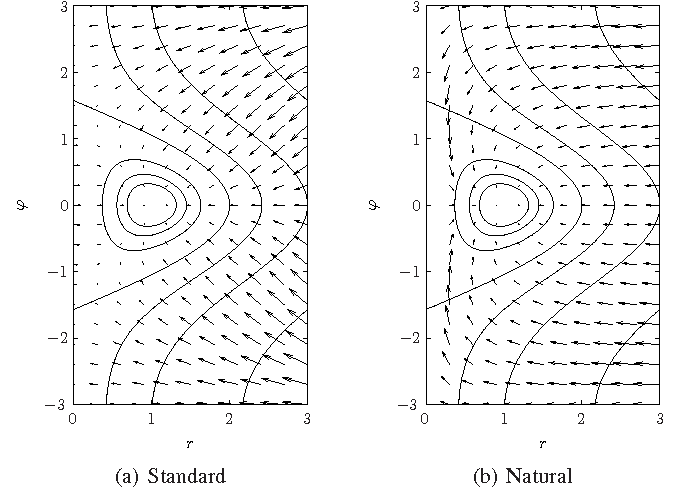
\includegraphics[width=0.52\textwidth]{vector_field}
    }       \label{fig:field}
    \subfigure[Training Paths]{
        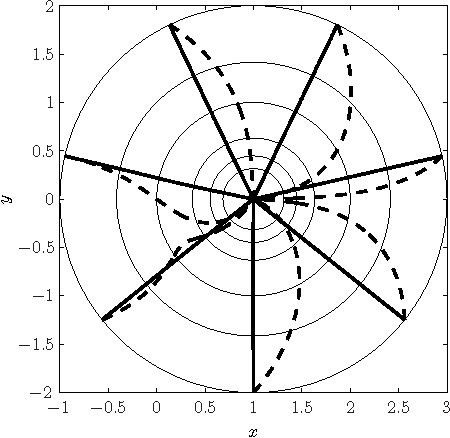
\includegraphics[width=0.38\textwidth]{training_trajectories}
    }        \label{fig:paths}
\end{figure}

{\let\thefootnote\relax\footnotetext{Figures and example taken from \cite{grondman2012survey}.}}

\end{frame}

\begin{frame}{Background on Natural Gradients: Fisher Information}

    \begin{itemize}
        \item Consider the case where $f$ is a probability distribution parameterized by $\theta$: ($f(\theta) = p(\vx | \vtheta)$). Then the correct metric tensor is the Fisher Information (FI) matrix:
        \begin{align*}
            \vF(\theta) = \int p(\vx | \vtheta) \nabla_\theta \log p(\vx | \vtheta) \nabla_\theta \log p(\vx | \vtheta)^\top d\vx
        \end{align*}
        \item \textbf{Interpretation}: FI is the expected (centered) second moment of the score function $\nabla_\theta \log p(\vx | \vtheta)$ and measures the information about parameters $\vtheta$ in the random variable $\vx$.
        \item A useful identity for the FI:
        \[ \int p_\theta(\vx) \nabla_\theta \log p_\theta(\vx) \nabla_\theta \log p_\theta(\vx)^\top d\vx = -\int p_\theta(\vx) \nabla^2_\theta \log p_\theta(\vx) d\vx \]
    \end{itemize}

\end{frame}

\begin{frame}{FI and the Policy Gradient Theorem}
    Let's return to policy gradients:
    \begin{align*}
        \nabla_\theta J(\pi_\theta) &= \int_\cS d^\pi(\bar \vs) \int_\cA \pi_\theta(\va | \bar \vs) \nabla_\theta \log \pi_\theta(\va | \bar \vs) \nabla_\theta \log \pi_\theta(\va | \vs)^\top \vw \ d\va d\bar \vs\\
        &= \int_\cS d^\pi(\bar \vs) \vF(\vtheta) \vw \ d\bar \vs
    \end{align*}
    The policy gradient clearly contains the FI of the policy conditioned for state $\vs$.
    Define the "average" FI:
        \[ \bar \vF(\theta) :=  \int_\cS d^\pi(\bar \vs) \vF(\vtheta) \ d\bar \vs \]
    If $\bar \vF(\theta)$ is the FI of an "appropriate" distribution, the natural gradient is:
    \[ \bar \vF(\theta)^{-1} \nabla_\theta J(\pi_\theta) = \vw \]
\end{frame}

\begin{frame}{Natural Policy Gradients: Trajectories}

    \begin{itemize}
        \item The probability of a trajectory $\vtau_{0:t}$ obtained when acting under the policy $\pi_\theta(\va | \vs)$ is:
        \[ p^\pi(\vtau_{0:t}) = d_0(\vs_0) \prod_{i=0}^t f(\vs_{i+1} | \vs_i, \va_i) \pi_\theta(\va_i | \vs_i) \]
        \item \textbf{Average reward:} it is straightforwad to show that $\bar \vF(\theta)$ is the FI of $\lim_{t \rightarrow \infty} p^\pi(\vtau_{0:t})$.
        \item \textbf{Discounted reward:} Peters et al. \cite{peters2003reinforcement} define a "discounted trajectory" distribution:
        \[ p_\gamma^\pi(\vtau_{0:t}) = p^\pi(\vtau_{0:t}) \left(\sum_{i=0}^n \gamma^i * \mathbbm{1}_{s_i, a_i} \right) \]
    \end{itemize}

\end{frame}

\begin{frame}{Natural Policy Gradients: Discounted Trajectory Distribution}
    Interpretations:
    \begin{itemize}
        \item \textbf{Probably Incorrect}: A single scaling factor on the distribution:
            \[ p_\gamma^\pi(\vtau_{0:t}) = p^\pi(\vtau_{0:t}) * \sum_{i=0}^t \gamma^i  \]
        \item \textbf{Closer}: A set of equivalent probability distributions with different un-normalized density functions:
             \[ p_\gamma^\pi(\vtau_{0:t}) = p^\pi(\vtau_{0:t}) \sum_{i=0}^t \gamma^i \mathbbm{1}_{s_i, a_i}(\vtau_{0:t})\]
    \end{itemize}

    Peters et al. \cite{peters2003reinforcement} prove that $\bar \vF(\theta)$ is the FI of the discounted trajectory distribution. Lets look carefully at their argument.

\end{frame}

\begin{frame}{Natural Policy Gradients: Statement}
    \textbf{Theorem 3 - Natural Policy Gradient:} \cite{peters2003reinforcement} The average FI information
    \[\bar \vF(\theta) = \int_\cS d^\pi(\bar \vs) \vF(\vtheta) \ d\bar \vs\]
    is the FI of the discounted trajectory distribution $p_\gamma^\pi(\vtau_{0:t})$.

    \textbf{Proof:}

    Recall the defintion of the trace distribution:
        \[ p^\pi(\vtau_{0:t}) = d_0(\vs_0) \prod_{i=0}^t f(\vs_{i+1} | \vs_i, \va_i) \pi_\theta(\va_i | \vs_i) \]
    The Hessian of the log probability is
        \[ \nabla^2_\theta \log p_\gamma^\pi(\vtau_{0:t}) = \sum_{i=0}^t \nabla^2_\theta \log \pi_\theta(\va_i | \vs_i) \]

\end{frame}

\begin{frame}{Natural Policy Gradients: Starting the Derivation}
    \textbf{Approach:} transform the expression for the FI of $p_\gamma^\pi(\vtau_{0:t})$ to match that for $\bar \vF(\theta)$:
    \begin{align*}
        \vF(\theta) &= \lim_{t \rightarrow \infty} \int p_\gamma^\pi(\vtau_{0:t}) \nabla_\theta \log p_\gamma^\pi(\vtau_{0:t}) \nabla_\theta p_\gamma^\pi(\vtau_{0:t})^\top d \vtau_{0:t}\\
        &= - \lim_{t \rightarrow \infty} \int p_\gamma^\pi(\vtau_{0:t}) \nabla^2_\theta \log p_\gamma^\pi(\vtau_{0:t}) d \vtau_{0:t}\\
        &= - \lim_{t \rightarrow \infty} \int p_\gamma^\pi(\vtau_{0:t}) \sum_{i=0}^t \nabla^2_\theta \log \pi(\va_i | \vs_i) d \vtau_{0:t}\\
        &= - \lim_{t \rightarrow \infty} \int \sum_{i=0}^t p_\gamma^\pi(\vtau_{0:t}) \nabla^2_\theta \log \pi(\va_i | \vs_i) d \vtau_{0:t}
    \end{align*}
\end{frame}

\begin{frame}{Natural Policy Gradients: Following Peters et al.}

    They appear to evaluate the indicator functions and then normalize the \textbf{sum} of density functions:
    {\small
    \begin{align*}
        \vF(\theta) &= - \lim_{t \rightarrow \infty} \int (1-\gamma) \sum_{i=0}^t \gamma^i p^\pi(\vtau_{0:t}) \nabla^2_\theta \log \pi(\va_i | \vs_i) d \vtau_{0:t}\\
        &= - \lim_{t \rightarrow \infty} \int (1-\gamma) \sum_{i=0}^t \gamma^i p^\pi(\vtau_{0:i}) \nabla^2_\theta \log \pi(\va_i | \vs_i) d \vtau_{0:i}\\
        &= - \lim_{t \rightarrow \infty} \int_\cS (1-\gamma) \sum_{i=0}^t \gamma^i p^\pi(\vs_i = \bar s) \int_\cA \pi_\theta(\va_i | \bar \vs) \nabla^2_\theta \log \pi(\va_i | \bar \vs) d \va_i d \bar \vs\\
        % PAPER RESUTLS
        &= - \int_\cS \gamma^i d^\pi(\vs = \bar s) \int_\cA \pi_\theta(\va | \bar \vs) \nabla^2_\theta \log \pi(\va | \vs) d \va d \bar \vs\\
        &= \int_\cS \gamma^i d^\pi(\vs = \bar s) \int_\cA \pi_\theta(\va | \bar \vs) \nabla_\theta \log \pi(\va | \vs) \nabla_\theta \log \pi(\va | \vs)^\top d \va d \bar \vs
    \end{align*} }
    Is this still defined w.r.t the correct distribution?
\end{frame}

\begin{frame}{Natural Policy Gradients: Getting Stuck}
    Normalizing the sum of density functions reweights the terms in the sum. Consider the same expression with pre-normalized densities:
    {\small \begin{align*}
        \vF(\theta) &= - \lim_{t \rightarrow \infty} \int \sum_{i=0}^t \frac{\gamma^i}{\gamma^i} p^\pi(\vtau_{0:t}) \nabla^2_\theta \log \pi(\va_i | \vs_i) d \vtau_{0:t}\\
        &= - \lim_{t \rightarrow \infty} \int \sum_{i=0}^t \frac{\gamma^i}{\gamma^i} p^\pi(\vtau_{0:i}) \nabla^2_\theta \log \pi(\va_i | \vs_i) d \vtau_{0:i}\\
        &= - \lim_{t \rightarrow \infty} \int_\cS \sum_{i=0}^t p^\pi(\vs_i = \bar s) \int_\cA \pi_\theta(\va_i | \bar \vs) \nabla^2_\theta \log \pi(\va_i | \bar \vs) d \va d \bar \vs\\
        &= - \lim_{t \rightarrow \infty} \int_\cS \sum_{i=0}^t p^\pi(\vs_i = \bar s) \int_\cA \pi_\theta(\va_i | \bar \vs) \nabla_\theta \log \pi(\va_i | \bar \vs) \nabla_\theta \log \pi(\va_i | \bar \vs)^\top d \va d \bar \vs
    \end{align*} }
    \textbf{Crux of the Issue:} the discounted trajectory distribution $p_\gamma^\pi(\vtau_{0:t})$.

\end{frame}

\begin{frame}{An Algorithmic Template for Natural Actor-Critic}

    \begin{enumerate}
        \item Choose initial parameters $\vw_0$, $\vtheta_0$.
        \item For $i = 0 ... $:
        \begin{enumerate}
            \item Update the Critic:
            \[\vw_{i+1} = \textbf{argmin}_w \int_\cS d^\pi(\bar \vs) \int_\cA \pi_\theta(\va | \bar \vs)\frac{1}{2}\left[Q^\pi(\bar \vs, \va) - R_w(\bar \vs, \va) \right]^2 d\va d\bar \vs\]
            \item Take a policy gradient step:
            \[\vtheta_{t+1} = \vtheta_{t} + \alpha_t \vw_{i+1} \]
        \end{enumerate}
    \end{enumerate}

    Convergence results for natural actor-critic algorithms depend on how the critic is updated. Convergence with probability 1 is guaranteed for some schemes.

\end{frame}

\begin{frame}[allowframebreaks]{References}
    \bibliographystyle{plain}
    \bibliography{refs}
\end{frame}

\end{document}
